% !TeX root = ..\main.tex
\section{Cơ sở lý thuyết}
\subsection{Lược đồ BPMN}
\subsubsection{BPMN là gì}

\hspace*{0.5cm}BPMN(Business Process Modeling Notation) là một lược đồ tập hợp các kí hiệu để mô hình hóa trực quan các quy trình nghiệp vụ xử lý . BPMN giúp các doanh nghiệp trực quan hóa các hoạt động và các luồng thông tin để thực hiện quy trình nghiệp vụ.
\begin{figure}[!htp]
	\centering
	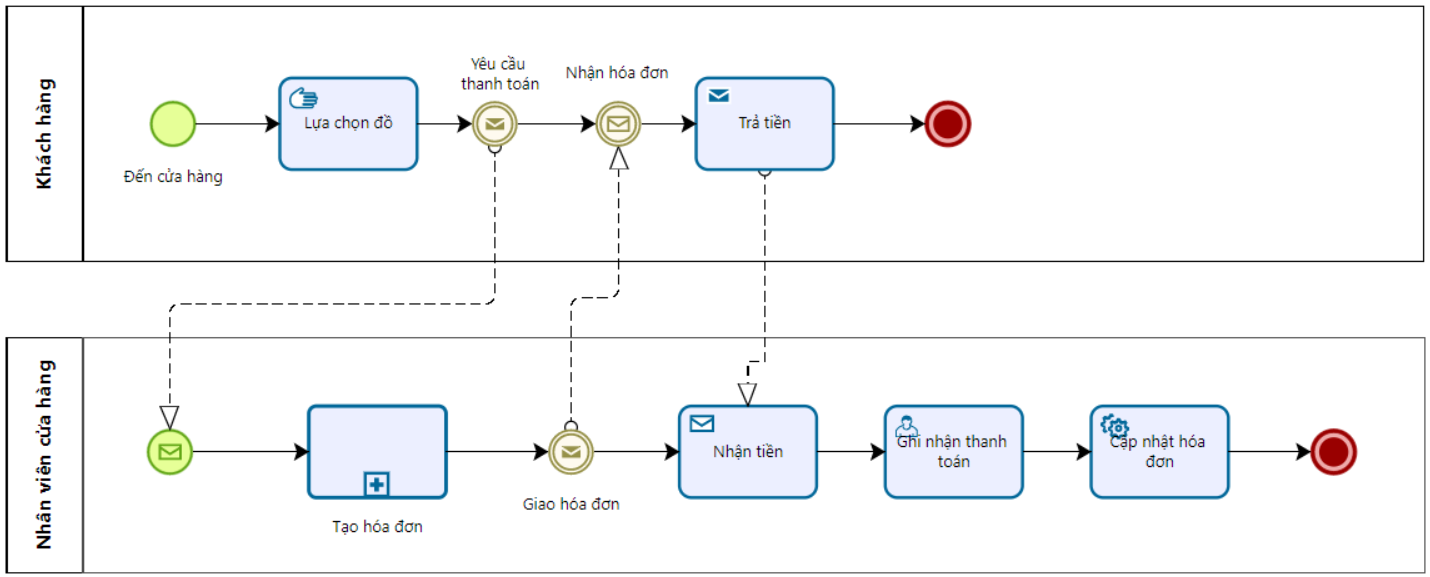
\includegraphics[width=10cm]{img/theory/BPMN/BPMN_sample.png}
	\newline
	\caption{Ví dụ về lược đồ BPMN}
\end{figure}



\subsubsection{Lợi ích của BPMN}
\begin{itemize}
	\item Giúp các bên liên quan có thể hiểu rõ quy trình nghiệp vụ của hệ thống
	\item Thu hẹp khoảng cách giửa bộ phận thiết kế và bộ phận nghiệp vụ
	\item Dễ dàng mô tả các nghiệp vụ phức tạp
\end{itemize}

\subsubsection{Các thành phần của BPMN}
\subsubsubsection*{Swimlane}
Swimlane bao gồm Pool và Lane:
\begin{itemize}
	\item Pool: Đại diện cho một tổ chức, phòng ban, một vai trò hoặc một hệ thống nào đó.
	\item Lane: Đại diện các cá nhân riêng lẻ, người sẽ làm các hoạt động cụ thể.
\end{itemize}

\begin{figure}[!htp]
	\centering
	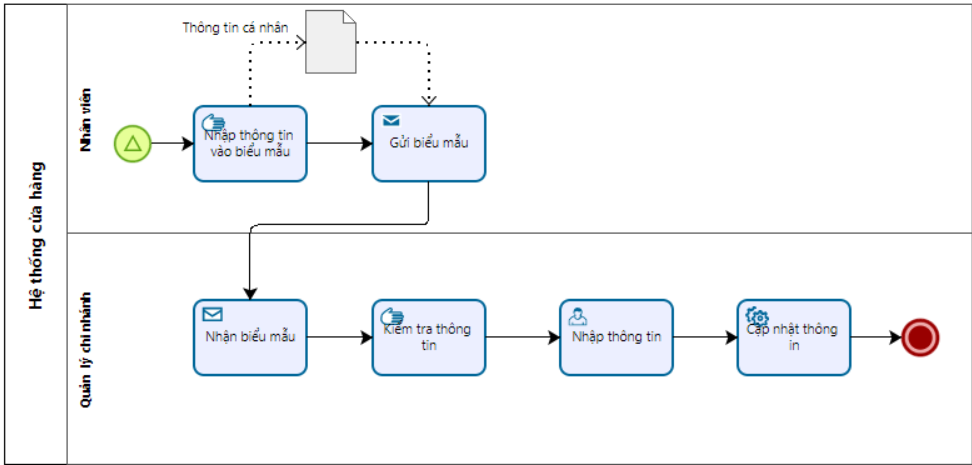
\includegraphics[width=10cm]{img/theory/BPMN/BPMN_swimlane.png}
	\newline
	\caption{Lược đồ BPMN bao gồm 1 pool(Hệ thống cứa hàng) và 2 lane (Nhân viên, Quản lý chi nhánh)}
\end{figure}

\subsubsubsection*{Activities}
Mô tả công việc trong quy trình, được kí hiệu bằng một kình chử nhật bo tròn 4 góc. Bao gồm 4 loại:
\begin{itemize}
	\item Task: Các việc nhỏ, đơn lẻ
	      \begin{figure}[!htp]
		      \begin{center}
			      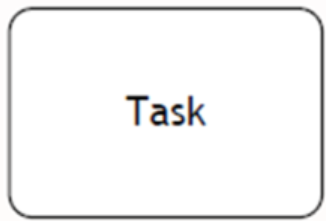
\includegraphics[width=2cm]{img/theory/BPMN/Task.png}
		      \end{center}
		      \caption{Task}
	      \end{figure}
	\item Event Sub-Process: Một quy trình con nằm trong một quy trình lớn, chức nhiều task
	      \begin{figure}[!htp]
		      \begin{center}
			      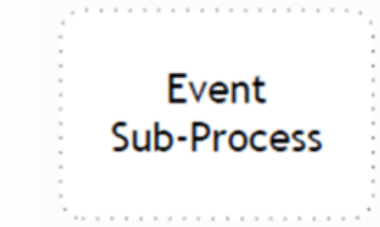
\includegraphics[width=2cm]{img/theory/BPMN/Event Sub-process.png}
		      \end{center}
		      \caption{Event Sub-Process}
	      \end{figure}
	\item Transaction: Các giao dịch, bao gồm các task nhỏ khác logic với nhau
	      \begin{figure}[!htp]
		      \begin{center}
			      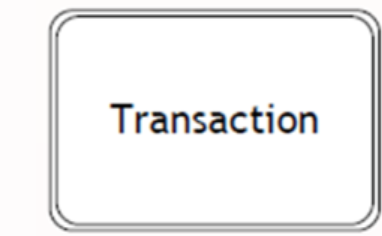
\includegraphics[width=2cm]{img/theory/BPMN/Transaction.png}
		      \end{center}
		      \caption{Transaction}
	      \end{figure}
	\item Call Activity: Gọi một quy trình khác đã được định nghĩa trong hệ thống, thay vì phải định nghĩa lại nhiều lần
	      \begin{figure}[!htp]

		      \begin{center}
			      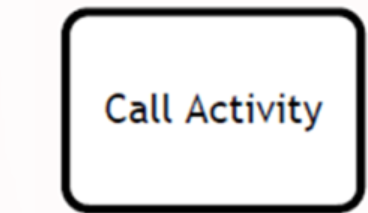
\includegraphics[width=2cm]{img/theory/BPMN/Call Activity.png}
		      \end{center}
		      \caption{Call Activity}
	      \end{figure}
\end{itemize}
\begin{flushleft}
	Các hình ảnh được lấy từ \url{https://thinhnotes.com/chuyen-nghe-ba/giai-ngo-cac-ky-hieu-bpmn/}
\end{flushleft}


\subsubsubsection*{Events}
Sự kiện là một điều gì đó xảy ra và có thể tác động đến quy trình nghiệp vụ. Một sự kiện có thể là bên ngoài hoặc bên trong nội bộ. Miễn là nó có tác động và ảnh hưởng trực tiếp đến quy trình nghiệp vụ. Các sự kiện thường được kí hiệu bằng hình tròn, bên trong có các kí hiệu về loại hình kích hoạt. Bao gồm các loại:
\begin{itemize}
	\item Start: Các sự kiện mở đầu quy trình nghiệp vụ
	\item Intermediate: Các sự kiện xảy ra giữa các quy trình nghiệp vụ
	\item End: Các sự kiện kết thúc quy trình nghiệp vụ
\end{itemize}
\begin{figure}[!htp]
	\begin{center}
		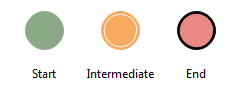
\includegraphics[width=6cm]{img/theory/BPMN/Event.png}
	\end{center}
	\caption{Các loại sự kiện trong BPMN}
\end{figure}
\begin{flushleft}
	Hình ảnh được lấy từ \textit{\url{https://www.edrawsoft.com/what-is-bpmn.html?gclid=Cj0KCQiAvqGcBhCJARIsAFQ5ke5U9xsSqU24T_1MgVtsStQ3wV0NbkzXcIY-rDCU8JAet5rGQMc6PyIaAgdxEALw_wcB}}
\end{flushleft}



\subsubsubsection*{Gateways}
Các cổng có nhiệm vụ chính là kiểm soát dòng chảy của quy trình nghiệp vụ. Cổng thường kí hiệu hình thoi, bên trong là kí hiệu các loại.
\begin{itemize}
	\item Start: Các sự kiện mở đầu quy trình nghiệp vụ
	\item Intermediate: Các sự kiện xảy ra giữa các quy trình nghiệp vụ
	\item End: Các sự kiện kết thúc quy trình nghiệp vụ
\end{itemize}
\begin{figure}[!htp]
	\begin{center}
		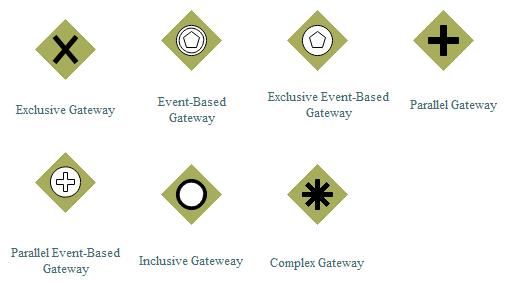
\includegraphics[width=8cm]{img/theory/BPMN/Gateway.png}
	\end{center}
	\caption{Các loại cổng phổ biến trong BPMN}
\end{figure}
\begin{flushleft}
	Hình ảnh được lấy từ \url{https://www.bacs.vn/vi/blog/kien-thuc/tong-quan-ve-bpmn-danh-cho-business-analyst-11002.html}
\end{flushleft}



%%%%%%%%%%%%%%%%%%%%%%%%%%%%%%%%%
\subsection{Ngôn ngữ BPEL}

%%%%%%%%%%%%%%%%%%%%%%%%%%%%%%%%%
\subsection{Chuyển đổi BPMN sang BPEL}